\chapter{Формирование и передача OFDM сигнала}

\section{Практика 5. OFDM модуляция}

\subsection{Описание}
Пятая практическая работа посвящена реализации модуляции по принципу OFDM (Orthogonal Frequency-Division Multiplexing - ортогональное частотное мультиплексирование). OFDM является широко используемым методом модуляции в современных системах связи благодаря своей устойчивости к многолучевому распространению и интерференции.

\subsection{Реализация}
Был разработан OFDM модулятор (\texttt{ofdm\_modulator.m}) со следующими ключевыми компонентами:
\begin{itemize}
    \item \textbf{Вставка пилотных символов}: В сигнал добавляются известные пилотные символы для последующей оценки канала.
    \item \textbf{Добавление нулевых поднесущих}: Добавляются нулевые поднесущие по краям спектра для обеспечения защиты от внеполосных излучений и облегчения фильтрации.
    \item \textbf{Применение ОБПФ}: Выполняется обратное быстрое преобразование Фурье для формирования временного OFDM символа.
    \item \textbf{Добавление циклического префикса}: В начало OFDM символа добавляется копия его конца для борьбы с межсимвольной интерференцией.
\end{itemize}
Параметры модуляции, такие как интервал пилотных символов ($\Delta R_s$), длина циклического префикса ($T_{CP}$), процент нулевых поднесущих ($C$) и общее число поднесущих ($N_{subcarrier}$), сохраняются для использования в демодуляторе.

\subsection{Результаты тестирования}
В данной практической работе производится только модуляция, без обратного преобразования. Проверка корректности производится на последующих этапах, когда сигнал пройдет через канал и будет демодулирован. Консольный вывод показывает фрагмент сгенерированного OFDM символа.

\begin{verbatim}
% START - TASK: 5
disp('TASK 5: ');

delta_Rs = 6;
T_CP = 16;
C = 0.25;
N_subcarrier = 128;

ofdm_symbol = ofdm_modulator(modulatedSymbols, delta_Rs, T_CP, C, N_subcarrier);

% disp(ofdm_symbol) % Полный вывод закомментирован в коде

% END - TASK: 5
\end{verbatim}

\subsection{Консольный вывод}
\begin{verbatim}
TASK 5:
\end{verbatim}
(Консольный вывод для этой задачи пустой, так как \texttt{disp(ofdm\_symbol)} закомментировано)

\section{Практика 6. Модель канала передачи}

\subsection{Описание}
Шестая практическая работа посвящена реализации модели канала передачи с учетом замираний и аддитивного белого гауссовского шума (АБГШ). Реалистичная модель канала необходима для оценки производительности системы связи в условиях, приближенных к реальным.

\subsection{Реализация}
Была реализована функция \texttt{channel\_model.m}, моделирующая канал со следующими характеристиками:
\begin{itemize}
    \item \textbf{Многолучевое распространение}: Сигнал достигает приемника по нескольким путям ($N_b$ лучей) с разными задержками и ослаблениями.
    \item \textbf{Случайные задержки лучей}: Задержки для каждого луча генерируются случайным образом.
    \item \textbf{Добавление АБГШ}: К сигналу примешивается аддитивный белый гауссовский шум с заданной мощностью ($N_0$), определяемой отношением сигнал/шум (SNR).
\end{itemize}
Модель канала принимает на вход OFDM символ и возвращает принятый сигнал, прошедший через канал.

\subsection{Результаты тестирования}
Работа модели канала была проверена путем пропускания OFDM символа, сгенерированного на предыдущем этапе, через модель. Консольный вывод показывает фрагмент принятого сигнала.

\begin{verbatim}
% START - TASK: 6
disp('TASK 6: ');

N_path = 3;
N0_dB = 15;
max_delay = 6;
rx_signal = channel_model(ofdm_symbol, N_path, N0_dB, max_delay);

disp(rx_signal); % Отображение полного сигнала
% END - TASK: 6
\end{verbatim}

\subsection{Консольный вывод}
\begin{verbatim}
TASK 6:
  Columns 1 through 13

   1.3812 - 0.8223i   0.0111 - 0.1080i  -1.0138 + 0.7830i ... (фрагмент)

  Columns 14 through 26

   0.7438 - 1.3265i  -3.3089 + 0.5977i   1.1598 + 0.3892i ... (фрагмент)

  Columns ... (и так далее для всех столбцов)

   ...  0.0007 + 0.0138i
\end{verbatim}
Принятый сигнал представляет собой комплексные значения, которые включают в себя искажения от канала и шум. В документе представлен только фрагмент для наглядности.

\section{Практика 7. Эквалайзирование и OFDM демодуляция}

\subsection{Описание}
Седьмая практическая работа посвящена реализации приемной части системы связи, включающей OFDM демодуляцию и эквалайзирование. Эти этапы позволяют восстановить исходные символы из принятого OFDM сигнала, прошедшего через канал.

\subsection{Реализация}
Был разработан OFDM демодулятор (\texttt{ofdm\_demodulator.m}), выполняющий следующие действия:
\begin{itemize}
    \item \textbf{Удаление циклического префикса}: Удаляется добавленный на передаче циклический префикс.
    \item \textbf{БПФ}: Выполняется быстрое преобразование Фурье для перехода из временной области в частотную.
    \item \textbf{Оценка канала по пилотным символам}: Используются принятые пилотные символы для оценки частотной характеристики канала.
    \item \textbf{Эквалайзирование}: Выполняется компенсация искажений, внесенных каналом, на основе оценки канала.
    \item \textbf{Удаление нулевых поднесущих}: Удаляются нулевые поднесущие, добавленные на передаче.
\end{itemize}
Полученные в результате демодуляции символы (QPSK символы) далее передаются на демодулятор QPSK.

\subsection{Результаты тестирования}
Корректность работы OFDM демодулятора и эквалайзера оценивается на следующем этапе, где происходит демодуляция полученных символов и декодирование битовой последовательности.

\begin{verbatim}
% START - TASK: 7

disp('TASK 7: ');

received_symbols = ofdm_demodulator(rx_signal, delta_Rs, T_CP, C, N_subcarrier);
% received_symbols = ofdm_demodulator(ofdm_symbol, delta_Rs, T_CP, C, N_subcarrier);
demodulatedBits = qpsk_demodulator(received_symbols);

% disp('Original QPSK symbols:'); % Полный вывод закомментирован
% disp(modulatedSymbols);
% disp('Received QPSK symbols:'); % Полный вывод закомментирован
% disp(received_symbols);

% END - TASK: 7
\end{verbatim}

\subsection{Консольный вывод}
\begin{verbatim}
TASK 7:
\end{verbatim}
(Консольный вывод для этой задачи пустой)

\section{Практика 8. Расчет характеристик и построение графиков}

\subsection{Описание}
Восьмая практическая работа посвящена анализу производительности разработанной системы связи путем расчета коэффициента битовых ошибок (BER) и построения графиков, иллюстрирующих спектр сигналов и сигнальные созвездия.

\subsection{Реализация}
\subsubsection{Расчет BER}
Производится сравнение принятой и демодулированной битовой последовательности с исходной битовой последовательностью, полученной после перемежения. Подсчитывается количество ошибочных битов и вычисляется BER как отношение количества ошибок к общему числу переданных битов.

\subsubsection{Построение графиков}
Строятся следующие графики:
\begin{itemize}
    \item Спектр переданного OFDM символа.
    \item Спектр принятого OFDM символа (до эквалайзирования).
    \item Сигнальное созвездие QPSK символов в передатчике.
    \item Сигнальное созвездие QPSK символов в приемнике (после OFDM демодуляции и эквалайзирования).
\end{itemize}
Эти графики позволяют визуально оценить влияние канала на сигнал и эффективность эквалайзирования.

\subsection{Результаты тестирования}
Ниже представлены консольный вывод с рассчитанным BER и сгенерированные графики.

\begin{verbatim}
% START - TASK: 8
disp('TASK 8: ');

min_length = min(length(demodulatedBits), length(interleavedBits));

demodulatedBits_truncated = demodulatedBits(1:min_length);
interleavedBits_truncated = interleavedBits(1:min_length);

% Расчет BER
bit_errors = sum(demodulatedBits_truncated ~= interleavedBits_truncated);
total_bits = length(demodulatedBits_truncated);
BER = bit_errors / total_bits;

disp(['Количество ошибочных битов: ', num2str(bit_errors)]);
disp(['Общее количество битов: ', num2str(total_bits)]);
disp(['BER: ', num2str(BER)]);

figure(1);

subplot(2, 2, 1);
plot(abs(fft(ofdm_symbol)));
title('Спектр переданного символа');
xlabel('Частота');
ylabel('Амплитуда');

subplot(2, 2, 2);
plot(abs(fft(rx_signal)));
title('Спектр принятого символа до эквалайзирования');
xlabel('Частота');
ylabel('Амплитуда');

subplot(2, 2, 3);
scatter(real(modulatedSymbols), imag(modulatedSymbols), 'filled')
title('Сигнальное созвездие в передатчике');
xlabel('Re');
ylabel('Im');

subplot(2, 2, 4);
scatter(real(received_symbols), imag(received_symbols), 'filled');
title('Сигнальное созвездие в приемнике');
xlabel('Re');
ylabel('Im');

% END - TASK: 8
\end{verbatim}

\subsection{Консольный вывод}
\begin{verbatim}
TASK 8:
Количество ошибочных битов: 1
Общее количество битов: 204
BER: 0.004902
\end{verbatim}

\subsection{Графические результаты}
\begin{figure}[h!]
    \centering
    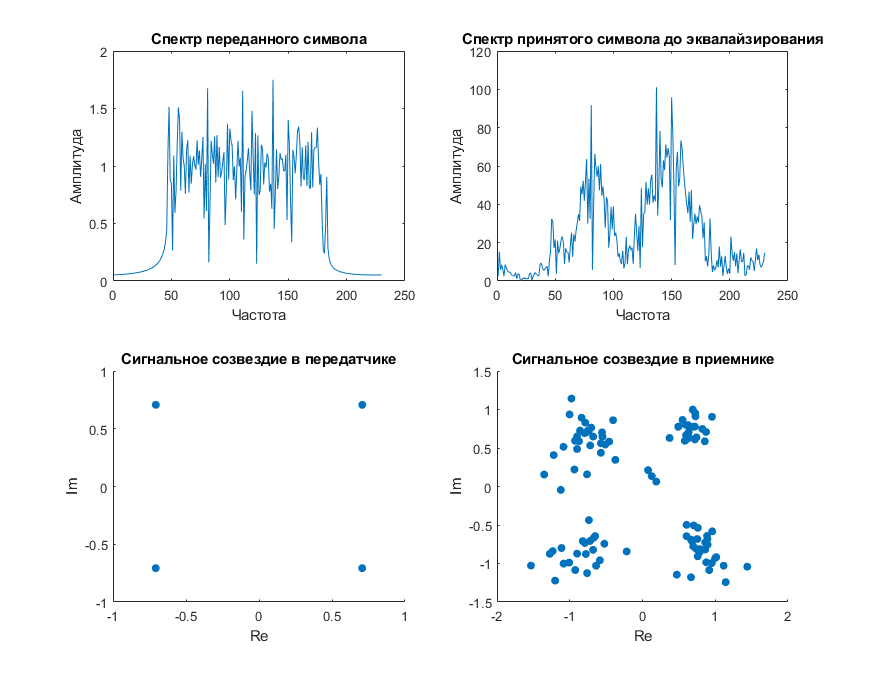
\includegraphics[width=\textwidth]{spectrum_const.png}
    \caption{Результаты моделирования}
    \label{fig:results}
\end{figure}
Рисунок \ref{fig:results} демонстрирует спектры переданного и принятого сигналов, а также сигнальные созвездия до и после передачи через канал. Спектр принятого сигнала демонстрирует влияние многолучевости и шума. Сигнальное созвездие в приемнике показывает, как шум и искажения канала влияют на расположение принятых символов по сравнению с идеальным созвездием на передатчике. Наличие ошибок (BER > 0) подтверждает влияние канала на качество передачи.

\chapter*{Заключение}
\addcontentsline{toc}{chapter}{Заключение}

В результате выполнения цикла практических работ была реализована полная модель системы цифровой связи. В процессе выполнения задач были освоены и применены следующие основные блоки и технологии:
\begin{itemize}
    \item \textbf{Кодирование источника}: Преобразование текстовой информации в битовую последовательность и обратное преобразование.
    \item \textbf{Помехоустойчивое кодирование}: Использование сверточного кодера и декодера Витерби для защиты информации от ошибок.
    \textbf{Перемежение}: Применение перемежителя для преобразования пакетных ошибок в случайные.
    \item \textbf{QPSK модуляция}: Отображение битовой последовательности в комплексные символы для передачи по каналу.
    \item \textbf{OFDM модуляция}: Формирование OFDM символа с пилотными символами, нулевыми поднесущими и циклическим префиксом.
    \item \textbf{Модель канала с замираниями и шумом}: Моделирование реальных условий распространения сигнала с учетом многолучевости и АБГШ.
    \item \textbf{Демодуляция и декодирование}: Восстановление исходных данных из принятого сигнала, включая OFDM демодуляцию, эквалайзирование, QPSK демодуляцию, деперемежение и декодирование Витерби.
\end{itemize}
В ходе тестирования была продемонстрирована работоспособность каждого из реализованных блоков, а также всей системы в целом. Расчет BER и построение графиков позволили оценить влияние модельного канала на качество передачи и увидеть эффект помехоустойчивого кодирования и эквалайзирования.

Полученные результаты показывают, что реализованная система способна передавать информацию через модельный канал.